\chapter{The Standard Model and Beyond}
\label{chap:theory}

The Standard Model of particle physics describes all
known fundemental particles and the interactions between them (with the exception
of the gravitational force). Developed over decades in the latter half of the 20$^\mrm{th}$
century, it has predicted experimental findings to an extraordinary degree of accuracy,
and represents one of the crowning achievements of modern science.
However, despite it successes, there are a number of known phenomena that cannot be
explained with the current theory, giving physicists reason to look for an expanded model.
In this chapter, we outline the Standard Model as it currently exists, discuss some
of the challenges that the model faces, and give a brief survey of proposed extensions to
the Standard Model that are relevant to this thesis.


\section{The Standard Model of particle physics}

The Standard Model (SM) is at its core a quantum field theory defined by a local 
$SU(3)\times SU(2)_L\times U(1)$ gauge symmetry. We will explain what exactly this means shortly 
(basically, each term gives rise to one of the three fundamental interactions), but for now we simply
describe all of the known particles and their properties.

\begin{figure}[ht]
  \begin{center}
    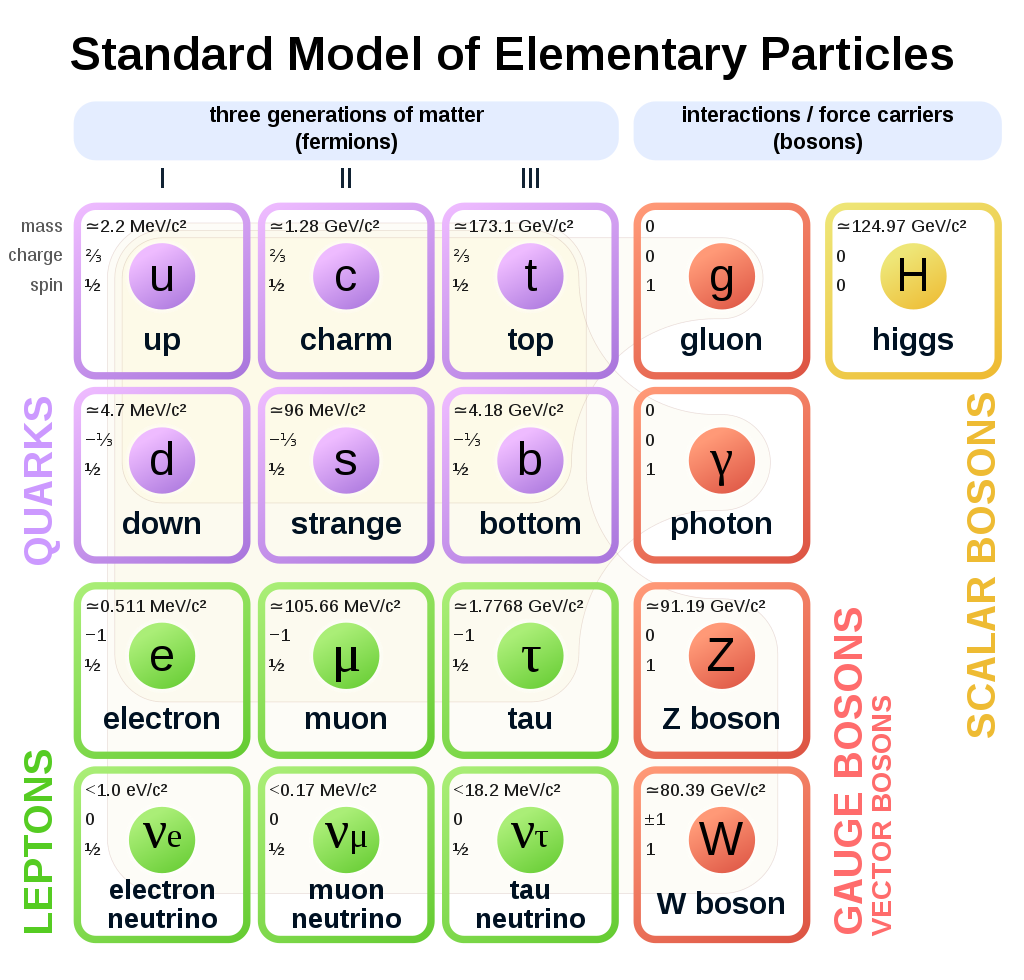
\includegraphics[width=0.70\textwidth]{figs/theory/standard_model.png}
    \caption{Diagram of all fundemental particles making up the Standard Model. There are 12 fermions (spin-\nicefrac{1}{2}), 
      consisting of six quarks (purple) and six leptons (green), 
      and divided into three generations. There are additionally four force-carrying vector bosons (spin-1),
      that couple to the fermions and give rise to the strong, weak, and electromagnetic interactions.
      Finally, the scalar Higgs boson, proposed in 1964 and discovered in 2012, provides the mechanism
      by which the other particles acquire mass. (Taken from \cite{SM_diagram})
            }
    \label{fig:sm}
  \end{center}
\end{figure}

\subsection{Fundamental particles}

Figure~\ref{fig:sm} shows all distinct particles in the SM, organized into groups.
On the left, in purple and green, are the 12 fundamental fermions, defined by the
value of their intrinsic angular momentum, or ``spin'', of \nicefrac{1}{2} (in units
of $\hbar$). By the spin-statistics theorem, fermions obey the Pauli exclusion principle,
meaning no two can occupy the same quantum state simultaneously.

The fermions are further defined by the various charges they carry (which determine how they
interact with the bosons, as we will see). In green are the six leptons, three with electric charge
of $-1$ (electron, muon and tau) and three that are electrically neutral (electron neutrino, muon
neutrino, and tau neutrino). In purple are the 6 types of quarks. The up-type quarks (up, charm, and top)
have electric charges of $+2/3$, and the down-type quarks (down, strange, and bottom) have electric
charges of $-1/3$. The quarks, in contrast to the leptons, carry color charge, meaning they
can interact via the strong interaction. All quarks and leptons carry weak isospin, meaning they can interact
via the weak interaction. Each of the fermions also has a corresponding antiparticle, which has the same
mass but opposite charges.

The fermions can be classified into three generations as indicated in the diagram, with masses
increasing in each generation (with the possible exception of the very light neutrinos, whose
masses are not precisely known). Due to various conservation laws arising from the allowed 
interactions, the first-generation particles are all stable, and hence form the building
blocks of matter. The strong interaction allows up and down quarks to strongly bind to
one another, forming protons (two ups and a down) and neutrons (two downs and an up).
The strong interaction further binds these into nuclei, which themselves bind to electrons via the electromagnetic
interaction to form atoms.

Moving to the right in the diagram, in red we have the four gauge bosons, which have spin-1
and which mediate the fundamental interactions. Their integer spin means they obey Bose statistics,
and are not constrained by the Pauli exclusion principle as are fermions. 
The gluon is massless, electrically neutral and mediates the strong
interaction. The photon is also massless and neutral and mediates the electromagnetic interaction. Finally,
the $W$ and $Z$ bosons are massive and mediate the weak interaction. The $Z$ is electrically neutral while 
the $W$ can carry charges of $\pm1$.

Finally, in yellow is the scalar (spin-0) Higgs boson. The Higgs mechanism was proposed in 1964 as an explanation
for how gauge bosons can acquire mass~\cite{Englert,Higgs,Guralnik}. A consquence of this mechanism is the prediction of a
scalar boson of undetermined mass, that couples to all SM particles proportionally to their masses.
The discovery of new boson of mass 125\GeV fitting these criteria (at least at the limits of current experimental precision) 
was announced by the CMS and ATLAS collaborations in July 2012~\cite{ATLAS:higgs,CMS:higgs}.

\subsection{Fundamental interactions}

Empirically, there are four known fundamental interactions, or ``forces'', between particles in our universe: 
the electromagnetic, weak, strong, and gravitational interactions. Gravity is understood
through Einstein's theory of general relativity, and is not (yet) integrated with our quantum understanding
of elementary particles. The other three interactions, on the other hand, are mathematically described by the
SM.

Essentially, each of the interactions arises by requiring that the Lagrangian describing the particle dynamics is
invariant under a certain \textit{local gauge transformation}. This means that if the particle fields are transformed
by some function that depends on spacetime position $x$, the Lagrangian is unchanged.
The full details are given in any quantum field theory textbook (e.g.~\cite{Peskin}), and we just give a brief
summary of the main ideas here.

The simplest example is the electromagnetic interaction. Starting with the Lagrangian of a free fermion
\be\label{eq:ferm_lagr}
\mathcal{L} = i\bar{\psi}\gamma^\mu\partial_\mu\psi - m\bar{\psi}\psi,
\ee
where $\psi$ is the spinor field of the fermion and $m$ is its mass,
we require that $\mathcal{L}$ is invariant under the local $U(1)$ transformation $\psi\to e^{-iq\theta(x)}\psi$.
The Lagrangian in Eq.~\ref{eq:ferm_lagr} is \textit{not} invariant under this transformation,
as we are left with an extra term proportional to $\partial_\mu\theta(x)$.

It turns out we can fix this by adding an extra term $-q\bar{\psi}\gamma^\mu\psi A_\mu$, where
$A_\mu$ is a new vector field that transforms by $A_\mu\to A_\mu+\partial_\mu\theta$. The new terms
introduced by the gauge transformation then cancel, and the Lagrangian is invariant.  The field
$A_\mu$ represents a new spin-1 particle, and to ensure that the Klein-Gordon equation is satisfied,
we must also add a ``free'' term. Doing this, it turns out the boson must be massless to ensure gauge invariance is
maintained.

So by requiring that the Lagrangian for a free fermion is invariant under a local $U(1)$ transformation,
we were forced to introduce a new massless, spin-1 boson that couples to the fermion via the term
$q\bar{\psi}\gamma^\mu\psi A_\mu$. This new boson is the photon, and this fermion coupling
is the fundamental interaction of quantum electrodynamics! The photon couples to any particle with
electric charge, represented by $q$ in the coupling term.

Feynman diagrams for the fundamental vertices of QED are shown in Fig.~\ref{fig:em_diagrams}.
On the left is the coupling of the photon to any charged fermion (leptons, with $|q|=1$, or
quarks, with $|q|=2/3$ or 1/3). The $W$ boson is also charged, and so couples to the photon,
but this vertex is best understood through electroweak unification discussed below.


\begin{figure}[ht]
  \addtolength{\abovecaptionskip}{5mm}
  \centering
  \vskip5mm
  \begin{fmffile}{feynman_diagrams/em_ferm}
  \begin{fmfgraph*}(40,25)
    \fmfleft{v1}
    \fmfright{o1,o2}
    \fmflabel{$e^-$}{o1}
    \fmflabel{$e^+$}{o2}
    \fmf{fermion}{o1,v2,o2}
    \fmf{photon,label=$\gamma$}{v1,v2}
  \end{fmfgraph*}
\end{fmffile}

  \begin{fmffile}{feynman_diagrams/em_w}
  \begin{fmfgraph*}(40,25)
    \fmfleft{v1}
    \fmfright{o1,o2}
    \fmflabel{$W-$}{o1}
    \fmflabel{$W+$}{o2}
    \fmf{boson}{o1,v2,o2}
    \fmf{photon,label=$\gamma$}{v1,v2}
  \end{fmfgraph*}
\end{fmffile}

  \caption{Fundemental vertices of the electromagnetic interaction. The photon couples to charged fermions (left)
    and the $W$ boson (right).
  }
  \label{fig:em_diagrams}
\end{figure}

To derive the strong interaction, we start with the assumption that quarks have ``color charge'',
which can be one of three values we refer to as red, green, and blue.
Then the free quark Lagrangian can be written
\be\label{eq:quark_lagr}
\begin{split}
\mathcal{L} &= \sum_{c=r,g,b} i\bar{q}_c\gamma^\mu\partial_\mu q_c - m\bar{q}_c q_c \\
&= i\bar{q}\gamma^\mu\partial_\mu q - m\bar{q}q
\end{split}
\ee
where $q$ is the quark spinor, $c$ represents the color charge, and we have introduced the shorthand
\be
q = \begin{pmatrix} q_r \\ q_g \\ q_b \end{pmatrix}, \;\;\;
\bar{q} = \left( \bar{q}_r \; \bar{q}_g \; \bar{q}_b \right).
\ee
This can also be summed over
the six flavors of quarks to describe all of them simultaneously.

The Lagrangian in Eq.~\ref{eq:quark_lagr} is already invariant under the global gauge transformation
$q\to Uq$, where $U$ is any $3\times3$ unitary matrix of determinant 1 (this group of matrices is called
$SU(3)$. It is not strictly necessary to require determinant 1, but we can factor out the determinant
as a separate $U(1)$ transformation, which would just re-derive QED for quarks). But if we further require
that the theory should be invariant under a \textit{local} $SU(3)$ transformation $U(x)$, we are again required
to add extra terms.

The details are quite a bit messier this time, as $SU(3)$ is a non-abelian group. But it turns out
that any matrix in $SU(3)$ can be written as $e^{-ig_s\boldsymbol\lambda\cdot\boldsymbol\alpha(x)}$, where
$\boldsymbol\lambda$ are the eight Gell-Man matrices and $\boldsymbol\alpha$ is an 8-dimensional vector,
and we are forced to add a term to the Lagrangian $g_s\bar{q}\gamma^\mu\boldsymbol(\boldsymbol\lambda\cdot\mathbf{A_\mu})q$.

This time, $\mathbf{A_\mu}$ is a vector of eight new spin-1 bosons (gluons), and this term represents the coupling of gluons
to quarks. In adding the kinetic terms for the gluons, we are again forced to make them massless, but this time,
due to the non-abelian nature of $SU(3)$, we are also forced to add additional terms that represent three- and four-gluon 
self-interaction vertices. The fundamental interactions for quantum chromodynamics are shown in Fig.~\ref{fig:strong_diagrams}.
The two on the right are the boson self-interactions, which are not present in QED, and are a feature of non-abelian
gauge theories.


\begin{figure}[ht]
  \addtolength{\abovecaptionskip}{5mm}
  \centering
  \vskip5mm
  \begin{fmffile}{feynman_diagrams/glu_q}
  \begin{fmfgraph*}(40,25)
    \fmfleft{v1}
    \fmfright{o1,o2}
    \fmflabel{$\bar{q}_j$}{o1}
    \fmflabel{$q_i$}{o2}
    \fmflabel{$g$}{v1}
    \fmf{fermion}{o1,v2,o2}
    \fmf{gluon}{v1,v2}
  \end{fmfgraph*}
\end{fmffile}

  \begin{fmffile}{feynman_diagrams/glu_tri}
  \begin{fmfgraph*}(40,25)
    \fmfleft{v1}
    \fmfright{o1,o2}
    \fmflabel{$g$}{o1}
    \fmflabel{$g$}{o2}
    \fmflabel{$g$}{v1}
    \fmf{gluon}{o1,v2,o2}
    \fmf{gluon}{v1,v2}
  \end{fmfgraph*}
\end{fmffile}

  \begin{fmffile}{feynman_diagrams/glu_quad}
  \begin{fmfgraph*}(40,25)
    \fmfleft{i1,i2}
    \fmfright{o1,o2}
    \fmflabel{$g$}{i1}
    \fmflabel{$g$}{i2}
    \fmflabel{$g$}{o1}
    \fmflabel{$g$}{o2}
    \fmf{gluon}{i1,v1,i2}
    \fmf{gluon}{o1,v1,o2}
  \end{fmfgraph*}
\end{fmffile}

    \caption{Fundemental vertices of the strong interaction. The gluon couples to a quark-antiquark
      pair, and also has 3- and 4-gluon self-interaction vertices. These are important for internal
      dynamics of hadrons as well as the hadronization of quarks and gluons at colliders.
            }
    \label{fig:strong_diagrams}
\end{figure}

The final interaction we must incorporate is the weak interaction. However, there are a number of difficulties
that did not arise for the electromagnetic and strong interactions.

\begin{figure}[ht]
  \addtolength{\abovecaptionskip}{5mm}
  \centering
  \vskip5mm
  \begin{fmffile}{feynman_diagrams/w_lep}
  \begin{fmfgraph*}(40,25)
    \fmfleft{v1}
    \fmfright{o1,o2}
    \fmflabel{$\bar{\nu}_\ell$}{o1}
    \fmflabel{$\ell^-$}{o2}
    \fmf{fermion}{o1,v2,o2}
    \fmf{photon,label=$W^-$}{v1,v2}
  \end{fmfgraph*}
\end{fmffile}

  \begin{fmffile}{feynman_diagrams/w_q}
  \begin{fmfgraph*}(40,25)
    \fmfleft{v1}
    \fmfright{o1,o2}
    \fmflabel{$\bar{q}_j$}{o1}
    \fmflabel{$q_i$}{o2}
    \fmf{fermion}{o1,v2,o2}
    \fmf{photon,label=$W$}{v1,v2}
  \end{fmfgraph*}
\end{fmffile}

  \begin{fmffile}{feynman_diagrams/z_ferm}
  \begin{fmfgraph*}(40,25)
    \fmfleft{v1}
    \fmfright{o1,o2}
    \fmflabel{$\bar{f}$}{o1}
    \fmflabel{$f$}{o2}
    \fmf{fermion}{o1,v2,o2}
    \fmf{photon,label=$Z$}{v1,v2}
  \end{fmfgraph*}
\end{fmffile}

    \caption{Fundemental vertices of the weak interaction. The $W$ boson can couple to a lepton
      and a same-generation neutrino, or a quark and anti-quark (most strongly within the same
      generation, but cross-generational couplings are possible via the CKM matrix).
      The $Z$ boson can couple to any fermion and its antiparticle. There are also
      boson self-interaction vertices ($WWZ$, $WWWW$, $WWZZ$) necessary for the self-consistency 
      of the theory, but they are less important practically.
            }
    \label{fig:weak_diagrams}
\end{figure}

\begin{figure}[ht]
  \addtolength{\abovecaptionskip}{5mm}
  \centering
  \vskip5mm
  \begin{fmffile}{feynman_diagrams/higgs_ferm}
  \begin{fmfgraph*}(40,25)
    \fmfleft{v1}
    \fmfright{o1,o2}
    \fmflabel{$\bar{f}$}{o1}
    \fmflabel{$f$}{o2}
    \fmf{fermion}{o1,v2,o2}
    \fmf{dashes,label=$H$}{v1,v2}
  \end{fmfgraph*}
\end{fmffile}

  \begin{fmffile}{feynman_diagrams/higgs_boson}
  \begin{fmfgraph*}(40,25)
    \fmfleft{v1}
    \fmfright{o1,o2}
    \fmflabel{$W,Z$}{o1}
    \fmflabel{$W,Z$}{o2}
    \fmf{boson}{o1,v2,o2}
    \fmf{dashes,label=$H$}{v1,v2}
  \end{fmfgraph*}
\end{fmffile}

  \begin{fmffile}{feynman_diagrams/higgs_gamma}
  \begin{fmfgraph*}(40,25)
    \fmfleft{v1}
    \fmfright{o1,o2}
    \fmflabel{$\gamma,g$}{o1}
    \fmflabel{$\gamma,g$}{o2}
    \fmf{fermion}{v2,v3,v4,v2}
    \fmf{photon}{v3,o1}
    \fmf{photon}{v4,o2}
    \fmf{dashes,label=$H$}{v1,v2}
  \end{fmfgraph*}
\end{fmffile}

    \caption{Interactions of the Higgs boson. It directly couples to any particle with mass,
      including fermions (left) and the $W$ and $Z$ bosons (middle). It cannot couple directly
      to massless particles such as the photon and gluon, but it may decay to these through loops
      of massive particles (right). The most likely particle in the loop is the top quark, since
      it is the heaviest option (thought it needs to be virtual, since $2m_t > m_H$).
            }
    \label{fig:higgs_diagrams}
\end{figure}


\section{Problems with the Standard Model}

\section{Theories of physics beyond the Standard Model}
\label{sec:bsm}
